\atstartofhistorysection
\section[Un peu d’histoire : degré et quantité  de chaleur]{Un peu d’histoire :\onlyamphibook{\\} degré et quantité  de chaleur}
\label{ch_histoire_quantite_chaleur_depondt}

\begin{center}\textit{Par Philippe Depondt\\ \begin{small}Université Pierre et Marie Curie, Paris\end{small}}\end{center}

	Dans la deuxième moitié du \textsc{xvii}\ieme\ siècle, on a commencé à se préoccuper de la distinction entre \emph{degré} de chaleur et \emph{quantité} de chaleur. C'était une question nouvelle qui n'a pu émerger que lorsqu'on a été capable de mesurer la température, ou le «~degré de chaleur~» d'un corps de façon fiable.

	Notre conception de la chaleur est en grande partie liée à la sensation de chaud ou de froid : on se brûle au contact d'eau bouillante, on a froid quand on prend un morceau de glace dans la main. On peut «~avoir~» plus ou moins chaud, ou plus ou moins froid, un objet chaud contient «~du chaud~», plus ou moins de chaud, tout ça, c'était un peu la même chose… Dans ce cadre, l'idée d'une matérialité de la chaleur, l'idée qu'une quantité de chaleur mesurable puisse être transférée d'un corps à un autre et induire des changements de température prévisibles et mesurables restait fort éloignée !

	\wf{Joseph Black} (1728-1799), à Édimbourg en Écosse, fait alors un pas en avant décisif : il constate que la neige ne fond pas instantanément alors que la température ambiante peut être largement supérieure à la température de fusion de la glace. Les congères de neige, même en plein soleil, peuvent mettre plusieurs jours avant de disparaître… Il se pose alors la question : quelle est la température de l’eau capable de faire fondre entièrement son propre poids de neige à~\SI{0}{\degreeCelsius} sans faire varier sa température ? L’expérience apporte la réponse : \SI{78}{\degreeCelsius} ! L'eau tiède s'est donc refroidie, alors que la neige est restée à la même température : les 78 degrés de chaleur apportés par l'eau tiède ont été incorporés dans la glace. La conclusion en est que la fusion de la neige a nécessité l'apport de ces 78 degrés de chaleur par l'eau liquide. Il appelle cette chaleur \vocab{la chaleur latente}~\cite{locqueneux1996}, pour la différencier de la chaleur \vocab{sensible} associée à des variations mesurables de température. Au-delà d'une expérience astucieuse et d'une interprétation brillante, il y a là l'apparition d'un nouveau concept.

	Black poursuit ses activités en faisant toute une série d'expériences de calorimétrie, mélanges d'eau à des températures différentes, mélanges de corps de nature différentes à différentes températures ; il met à chaque fois en évidence que la chaleur spécifique dépend de la nature du corps :
	
	\onlyframabook{\begin{quote}}%handmade
	\onlyamphibook{\begin{historyquote}}
		Nous devons, en conséquence, conclure que différents corps, bien qu’ils soient de la même taille ou même du même poids, lorsqu’ils sont réduits à la même température ou degré de chaleur, quoi que cela puisse bien être, peuvent contenir des quantités très différentes de la matière de chaleur ; lesquelles quantités sont nécessaires pour les amener à ce niveau, ou équilibre, l’un avec l’autre.
	\begin{flushright}\vspace{-0.5em}Joseph Black, 1807~\cite{black1807}\end{flushright}
	\onlyamphibook{\end{historyquote}}
	\onlyframabook{\end{quote}}

	Il ne fait pas d'hypothèse sur la nature de cette chaleur qu'il a caractérisée. Pour la plupart de ses contemporains, cependant, son apparente conservation indique qu'il s'agit d'un fluide matériel dépourvu de masse que Lavoisier appellera plus tard le \vocab{calorique}. Cette matière peut être transférée d'un corps à l'autre pour élever la température de celui qui la reçoit et abaisser celle de celui qui la cède : certains corps (l'eau par exemple) en contiennent, à une température donnée, plus que d'autres (comme l'huile), ce qui se traduit par des chaleurs spécifiques différentes. De son côté, Black pensait que la fusion d'un solide ou la vaporisation d'un liquide pouvait être une espèce de combinaison chimique du fluide calorique et de la matière : le calorique disparaîtrait alors en tant que tel et deviendrait ainsi «~latent~».

	\begin{figure}[h!]
		\begin{center}
			\onlyframabook{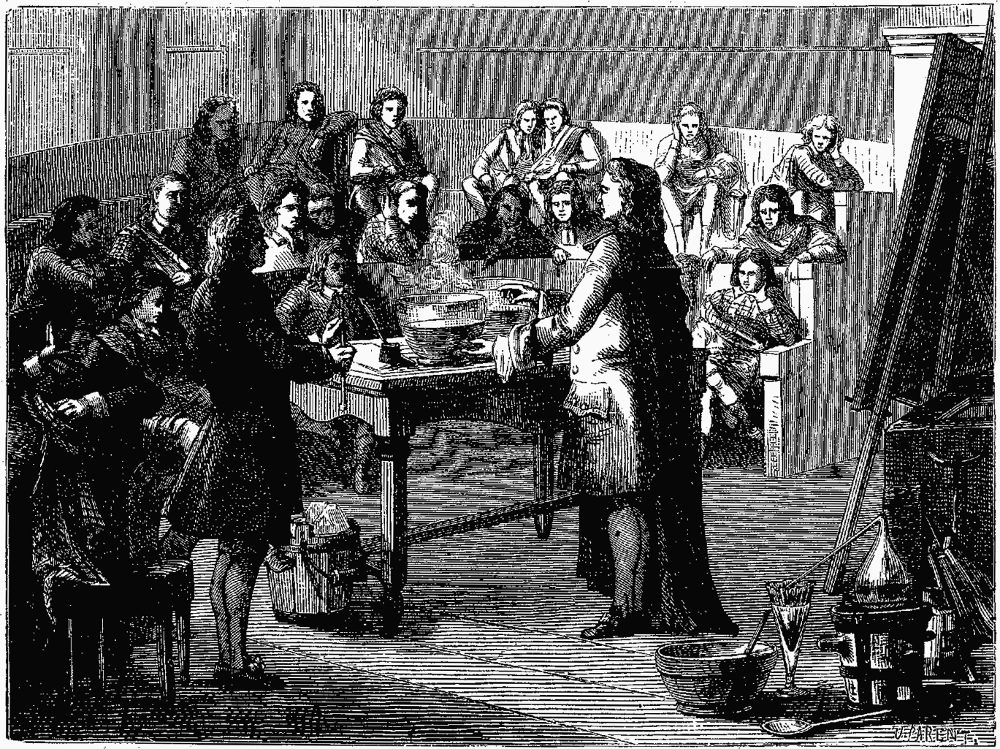
\includegraphics[width=10cm]{images/joseph_black_calorique_latent.png}}%handmade
			\onlyamphibook{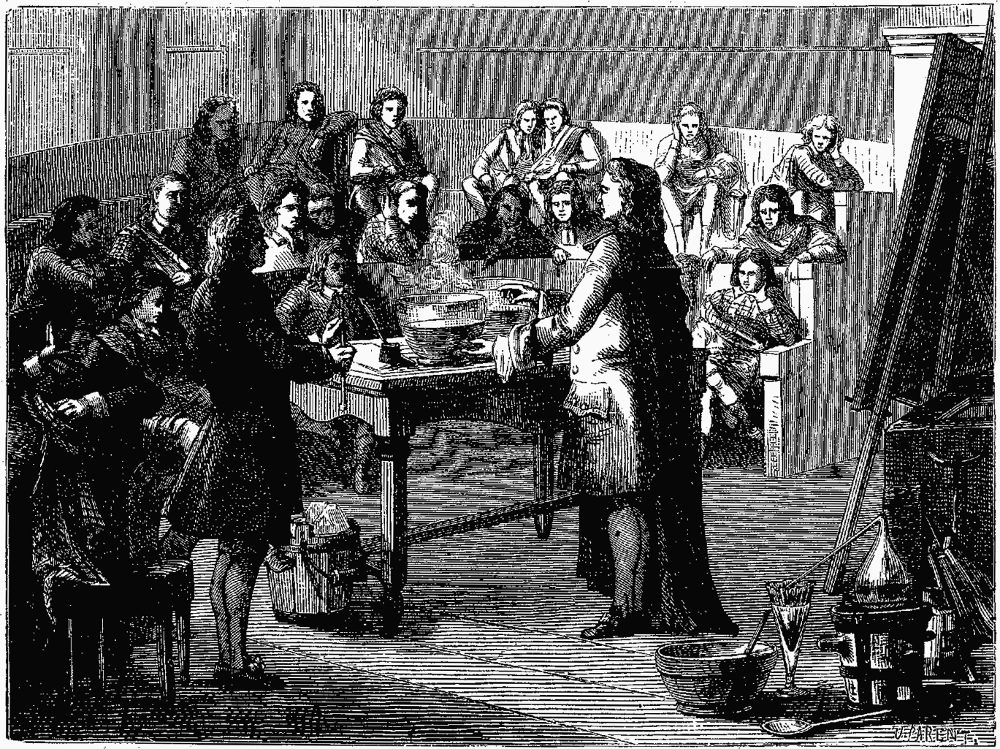
\includegraphics[width=0.85\columnwidth]{images/joseph_black_calorique_latent.png}}
			\supercaption{Joseph Black procédant à une expérience sur la chaleur latente pendant un cours universitaire à Édimbourg. On imagine qu’il n’avait aucun mal à passionner les étudiants, puisqu’il s’agit de thermodynamique…}%
			{\wcfile{T1- d083 - Joseph Black fait l'expérience du calorique latent.png}{gravure} d’auteur inconnu publiée par Louis Figuier en 1867 (\pd)}
			\label{fig_black_calorique_latent}
			\onlyamphibook{\vspace{-2cm}}%handmade
		\end{center}
	\end{figure}
\atendofhistorysection
